\subsection{CPU}

A \ac{cpu} is a digital processor that executes instructions of a computer program. These instructions are specific to the processors architecture and may perform arithmetic operations or interface with memories or external components. As the name suggests, it is the central component in most digital computing systems.

\subsubsection{Operation}

The main purpose of a \ac{cpu} is to sequentially execute a set of instructions stored in some memory. An instruction performs a single action, modifying the state of the processor accordingly. For example, it may calculate the product or sum of two numbers and store them in some memory. Or it may transfer data between main memory and internal registers. This sequence of instructions is called the computer program. In most architectures, it is easily modifiable, making the computer programmable.

\subsubsection{Instruction Cycle}

The execution of a program is typically done in discrete, synchronous steps, as dictated by one or more clock signals. Each edge of these clock signals advances the progress of the instruction cycle. The instruction cycle typically consists of the three phases of fetching, decoding and executing an instruction. In the fetch phase, the processor retrieves an instruction from program memory. Afterwards, in the decoding phase, the semantics of the fetched instruction are analysed and the internal state of the \ac{cpu} is setup. This involves extracting any operands and setting up the control signals that dictate what is done during the execution phase. In that phase, the desired operation is performed and any results are stored back into the relevant memories. These three phases form the instruction cycle. Each of the phases may take one or more clock cycles, although there are designs that combine some or all phases into shared ones. There are also processors that do not have a global clock signal for synchronisation. These designs are called ``asynchronous processors''. However, synchronous processors are by far more prevalent. In such designs, the asynchronous sections are communicating through synchronous gates, usually registers. This allows the asynchronous sections to be of different complexity, with different propagation delays.

\subsubsection{Structure}

A \ac{cpu} can be subdivided into its functional groups. 
A typical, minimalistic \ac{cpu} has 3 main components:

\begin{itemize}
    \item \ac{alu}
    \item Register File
    \item Control Unit
\end{itemize}

The \ac{alu} is an asynchronous circuit that performs logical and arithemtic operations. Its inputs are one or more operands, loaded from either an external memory, internal memories such as registers or directly from a given instruction. It performs an operation and outputs the result. Most \acp{alu} also output additional information in the form of one or more flags. These flags include auxiliary information such as the carry-out bit for addition operations or a bit indicating whether the result is zero or negative. These flags are usually saved to some register so they can be inspected in future instructions.

The register file consists of a set of registers that can be used to store temporary results. Each register stores a certain, fixed number of bits in a synchronous manner. Registers function as the synchronising instance between asynchronous circuits. While a \ac{cpu} may contain numerous registers used for equally numerous purposes, the register file consists only of general purpose registers exposed to programmers. Other uses for registers include a program counter, memory address registers, external flag registers and \ac{io} registers. These registers may only be indirectly or not at all visible to the programmer.

The control unit contains the logic necessary to orchestrate all other components and circuits within the \ac{cpu}. For example, depending on the current instruction, it tells the \ac{alu} whether to use an operand from memory or from a register or whether to update the flags register or not. It does this by mapping the instruction opcode to a set of control flags, which in turn control circuitry that sets up the datapath. It also contains the circuitry controlling the state of the instruction cycle.

\autoref{fig:cpu_structure} shows the composition of a \ac{cpu} from these three components, as well as the external interfaces that interact directly with it. The \ac{alu} and register file combine to form the processor, whose actions are then orchestrated by a control unit.

\begin{figure}[h!]
    \centering
    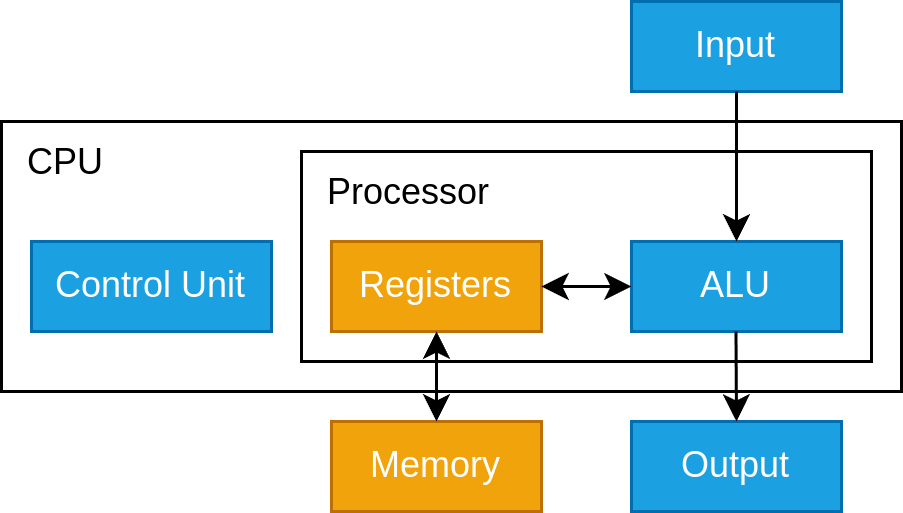
\includegraphics[width=0.7\textwidth]{images/drawio/cpu_structure.png}  % Replace with your image file
    \caption{Structure of register based CPU; arrows represent data flow. Blue components represent asynchronous circuitry, orange compontents represent synchronous circuitry. (Modified from Wikipedia, aggregated data flow arrows \cite{wikipedia_cpu})}
    \label{fig:cpu_structure}
\end{figure}

The \ac{alu} is the device performing the actual computations within a processor. It contains digital logic circuits that perform arithmetic such as addition, subtraction, multiplication, division or logical operations such as AND, OR, NOT, etc. When a programmer requests the \ac{cpu} to calculate some mathematical formula, it is this device that does the calculations. It is asynchronous does not require any clock signal. 


